\documentclass[10pt,twocolumn,letterpaper]{article}

\usepackage{cvpr}
\usepackage{times}
\usepackage{epsfig}
\usepackage{graphicx}
\usepackage{amsmath}
\usepackage{amssymb}
\usepackage{mathtools}
\usepackage{multicol}

\DeclarePairedDelimiter\abs{\lvert}{\rvert}%

% Include other packages here, before hyperref.

% If you comment hyperref and then uncomment it, you should delete
% egpaper.aux before re-running latex.  (Or just hit 'q' on the first latex
% run, let it finish, and you should be clear).
\usepackage[breaklinks=true,bookmarks=false]{hyperref}

\cvprfinalcopy % *** Uncomment this line for the final submission

\def\cvprPaperID{****} % *** Enter the  Paper ID here
\def\httilde{\mbox{\tt\raisebox{-.5ex}{\symbol{126}}}}

% Pages are numbered in submission mode, and unnumbered in camera-ready
\setcounter{page}{1}
\begin{document}

%%%%%%%%% TITLE
\title{EE3-23: Coursework for Introduction to Machine Learning}

\author{Douglas Brion\\
Imperial College London\\
CID: 01052925\\
{\tt\small db1415@ic.ac.uk}
}

\maketitle
%\thispagestyle{empty}


%%%%%%%%% BODY TEXT
\section{Introduction}

This report examines different approaches to predicting wine quality using the Wine Quality~\cite{WineQuality} dataset. This is a large dataset containing 4898 samples of white wines and 1599 of red. Throughout this report wine quality is examined using regression, attempting to predict the quality of a wine from various input parameters. Multiple learning methods are implemented, discussed and compared in order to obtain a predictor with the smallest test error possible.

All code for this report was written in Python and used the library Pandas~\cite{mckinneypandas} for importing and manipulating data and Tensorflow~\cite{tensorflow2015-whitepaper} for creating and training models to predict the data.

%-------------------------------------------------------------------------
\section{Data Preparation}
Both red and white wine datasets were available and it was decided to combine both into a single dataset consisting of 6497 samples in order to learn how to predict the quality of either a red or white wine. 

The data provided in the now combined dataset was not normalised, therefore each attribute was normalised with respect to it's mean and standard deviation. Outliers over a threshold of $Thres = 5$ from each attribute were then removed to reduce noise in the dataset for training. This altered data was output to 
\verb|winequality-fixed.csv|.

\begin{figure}[h]
	\begin{center}
		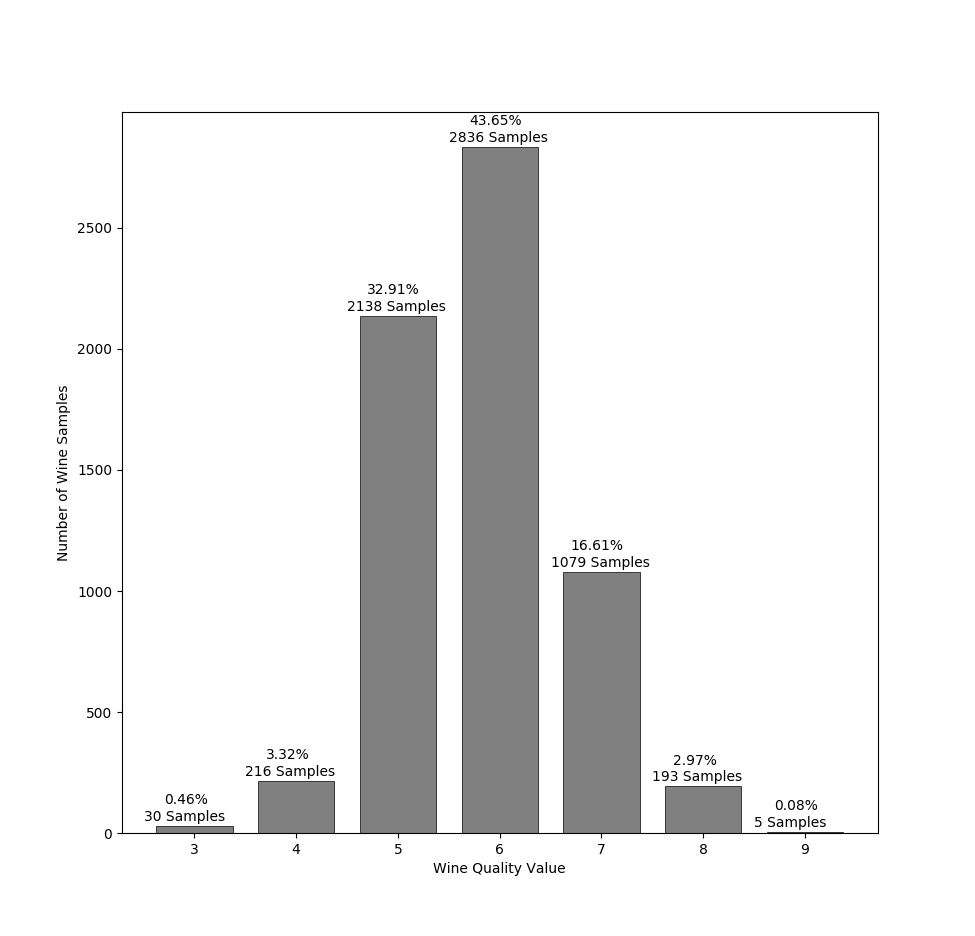
\includegraphics[width=0.9\linewidth]{img/samples.png}
	\end{center}
	\caption{The histogram for both white wine and red wine qualities.}
	\label{fig:hist}
\end{figure}


\begin{table}[h]
	\begin{center}
		\begin{tabular}{|l|c|c|c|c|}
			\hline
			Attributes & Mean & Std & Min & Max \\
			\hline
			fixed acidity & 7.22 & 1.30 & 3.80 & 15.9 \\
			volatile acidity & 0.34 & 0.16 & 0.08 & 1.58 \\
			citric acid & 0.32 & 0.15 & 0.00 & 1.66 \\
			residual sugar & 5.44 & 4.76 & 0.60 & 65.8 \\
			chlorides & 0.06 & 0.04 & 0.01 & 0.61 \\
			free sulfur dioxide & 30.5 & 17.8 & 1.00 & 289 \\
			total sulfur dioxide & 116 & 56.5 & 6.00 & 440 \\
			density & 0.99 & 0.00 & 0.98 & 1.04 \\
			pH & 3.22 & 0.16 & 2.72 & 4.01 \\
			sulphates & 0.53 & 0.15 & 0.22 & 2.00 \\
			alcohol & 10.5 & 1.19 & 8.00 & 14.9 \\ 
			\hline
		\end{tabular}
	\end{center}
	\caption{The attribute statistics before normalisation and removal of outliers.}
	\label{tab:attributes}
\end{table}

\begin{table}[h]
	\begin{center}
		\begin{tabular}{|l|c|c|c|c|}
			\hline
			Attributes & Mean & Std & Min & Max \\
			\hline
			fixed acidity & -0.012 & 0.965 & -2.635 & 4.848 \\
			volatile acidity & -0.005 & 0.984 & -1.577 & 4.800 \\
			citric acid & -0.002 & 0.990 & -2.193 & 4.689 \\
			residual sugar & -0.004 & 0.983 & -1.018 & 4.331 \\
			chlorides & -0.049 & 0.740 & -1.343 & 4.966 \\
			free sulfur dioxide & -0.008 & 0.968 & -1.664 & 4.957 \\
			total sulfur dioxide & -0.001 & 0.998 & -1.942 & 4.437 \\
			density & -0.004 & 0.979 & -2.530 & 2.999 \\
			pH & 0.000 & 1.000 & -3.101 & 4.923 \\
			sulphates & -0.017 & 0.936 & -2.092 & 4.898 \\
			alcohol & 0.000 & 1.000 & -2.089 & 3.696 \\ 
			\hline
		\end{tabular}
	\end{center}
	\caption{The attribute statistics after normalisation and removal of outliers.}
	\label{tab:normalised}
\end{table}

The goal of this project will be to find a predictor with the best regression performance.

\subsection{Learning approach}

For consistency all the different regressions performances of each model with varying parameters and training cost functions will be measured using the same error metric, the Huber Loss function. This is a good loss function for this regression problem as it is robust to outliers, for if the difference between the real and predicted value is small it will be squared, if large, the absolute value will be taken.

\begin{equation}
L_H = \begin{cases}
\sum_{i = 1}^{n} \frac{1}{2} (y_i - f(x_i))^2, & for \abs{y_i - f(x_i)} \leq \delta. \\
\sum_{i = 1}^{n} \delta \abs{y_i - f(x_i)} - \frac{1}{2} \delta^2, & otherwise.
\end{cases}
\end{equation}

This shall be used on the test error of each of the models for comparison as each model will required a different training error.

To validate which model is best they will also be tested using the Mean Absolute Deviation error metric (MAD) which is often used to test regression performance.

K-fold cross validation~\cite{CrossValidation}, where data is divided into K parts and with one part being tested at a time and remaining data used for training, gives robust and reliable estimates of the performance of the given model, although results in an increased computation time.

\section{Baseline Predictors}
Several baseline predictors have been implemented and trained on the data. 

A linear regression program was written in Python using Tensorflow~\cite{tensorflow2015-whitepaper}. This linear model used an iterative method to alter the weights, with multiple loss functions tested. This proved useful as a framework for the more advanced algorithms implemented later on.

For linear regression 2 basic loss functions were implemented first.

\subsection{L1 loss function}
The L1 loss function, least absolute deviations, tries to minimise the absolute difference between the predicted and real values. The sum of all the differences for all the samples can be described as follows:

\begin{equation}
L_1 = \sum_{i = 1}^{n} \abs{y_i - f(x_i)}
\end{equation}

This is a fairly robust loss function which is not that affected by outliers.

\begin{figure}[h]
	\begin{center}
		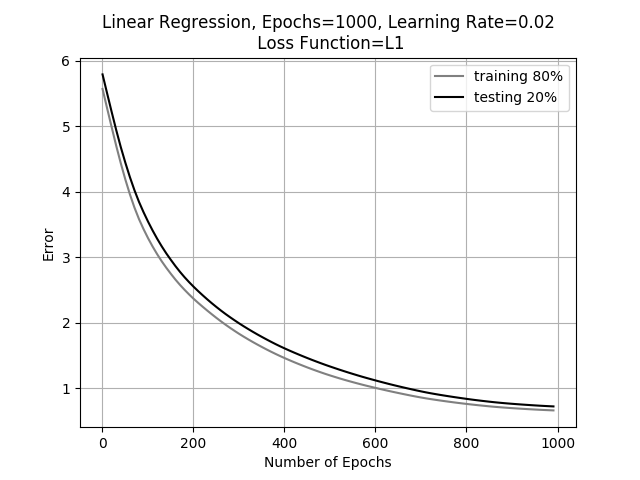
\includegraphics[width=0.9\linewidth]{img/l1loss.png}
	\end{center}
	\caption{Training Error = $\sum_{i = 1}^{n} \abs{y_i - f(x_i)}$ (L1 loss), Epochs = 1000, Learning Rate = 0.02}
	\label{fig:l1loss}
\end{figure}

\subsection{L2 loss function}
The L2 loss function, least square error, minimises the square difference between the predicted and real values. This value is much large than that of L1 loss and therefore is more affected by outliers, however, will optimise the predictor faster.

\begin{equation}
L_1 = \sum_{i = 1}^{n} (y_i - f(x_i))^2
\end{equation}

\begin{figure}[h]
	\begin{center}
		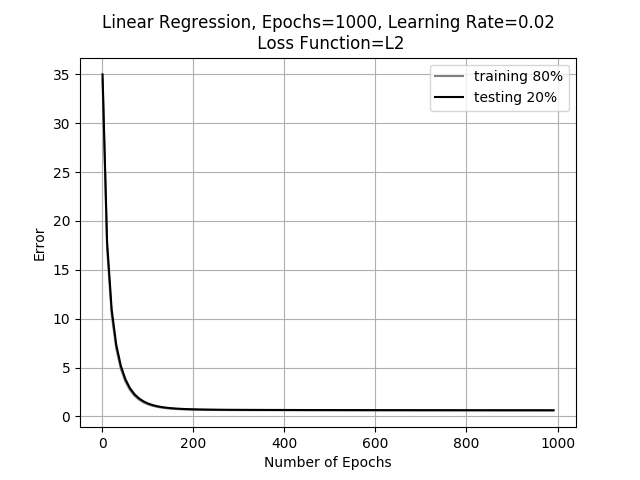
\includegraphics[width=0.9\linewidth]{img/l2loss.png}
	\end{center}
	\caption{Training Error = $\sum_{i = 1}^{n} (y_i - f(x_i))^2$ (L2 loss), Epochs = 1000, Learning Rate = 0.02}
	\label{fig:l2loss}
\end{figure}

Notice how the predictor using the L2 loss function in \ref{fig:l2loss}. minimises the error much faster than the L1 loss in \ref{fig:l1loss} and as outliers have been removed in data preparation the L2 loss is quite robust.

As the epochs are increased the optimiser is able to reduce the loss until no improvements can be made. The learning rate also greatly affects the rate at which the loss is minimised. However, if the learning rate is too high the predictor will not improve on the training data, as can be seen in \ref{fig:break}.

\begin{figure}[h]
	\begin{center}
		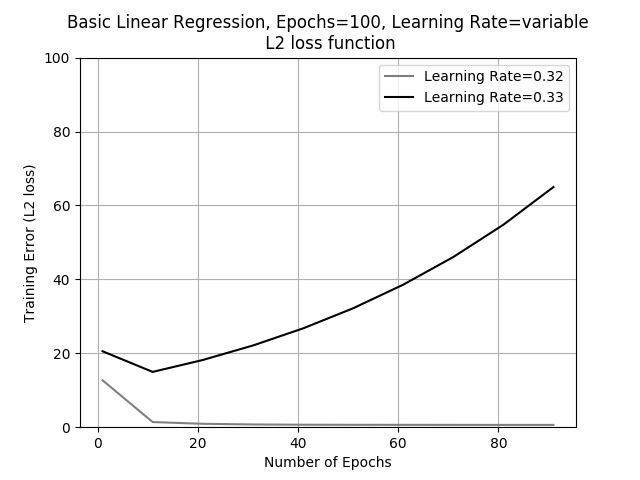
\includegraphics[width=0.9\linewidth]{img/linrbreak.png}
	\end{center}
	\caption{Training Error = $\sum_{i = 1}^{n} (y_i - f(x_i))^2$ (L2 loss), Epochs = 100, Learning Rate = variable}
	\label{fig:break}
\end{figure}

\subsection{Improvements}
These relatively simple models can be improved upon by adding regularisation. Regularisation is a technique used to prevent over fitting the data. Both L1 and L2 regularisation have been implemented, being the sum of the weights and sum of the square weights respectively. The regularisation term is added to the loss function, the terms for L1 and L2 look as follows:

\noindent\begin{minipage}{.5\linewidth}
	\begin{equation}
	L_{1reg} = \lambda \sum_{i = 1}^{n} \abs{w_i}
	\end{equation}
\end{minipage}%
\begin{minipage}{.5\linewidth}
	\begin{equation}
	L_{2reg} = \lambda \sum_{i = 1}^{n} w_i^2
	\end{equation}
\end{minipage}

\section{More Advanced Algorithms}

\subsection{Neural Network}
The neural network implemented as a predictor for this project had 3 layers, 1 input, 1 hidden and 1 output. A single hidden layer was chosen as an increase in hidden layers did not result in a significant increase in predictor performance although it did lengthen training time.

The number of nodes in the hidden was chosen using a heuristic of the number being the mean of the input and output layers, in this case resulting in 6 nodes.

Each layer could be assigned when the network is constructed to have a specific activation function such as: TanH, Sigmoid, ReLU, SeLU and Softmax. It was found that during training a hidden ReLU resulted in the best out of sample test error and therefore was chosen. 

Neural networks have an advantage over standard linear regression that they can model non-linearities automatically however they are more likely to overfit the data so observing the out of sample error is especially important.

\subsection{Support Vector Regression}
The goal for a support vector regression (SVR)~\cite{Cortes1995} predictor is to find a predication $f(x)$ like our other predictors however it should have at most $\epsilon$ deviation from the real value $y_i$ for all the in sample data.

The loss function for SVR is as follows:

\begin{equation}
L_{SVR} = max(0, \sum_{i = 1}^{n} \abs{y_i - f(x_i)} - \epsilon)
\end{equation}

This loss function is known as the hinge loss.

\subsection{Elastic Net Regularisation}



{\small
\bibliographystyle{ieee}
\bibliography{egbib}
}

\end{document}
